\chapter{Accelerating the inference on FPGA} \label{chap:fpga}
%
%
As said in Chapter \ref{chap:intr}, \acrshort{fpga} is a promising platform for the acceleration of \acrshort{cnn}s. According to \textcite{mittal_survey_2014}, \acrshort{fpga}s provide higher energy efficiency than both \acrshort{gpu}s and \acrshort{cpu} and a higher performance than \acrshort{cpu}s. Besides, \acrshort{fpga}s are very flexible hardware that can be tailored for each particular \acrshort{nn} \cite{vestias_fast_2019}. Furthermore, we can even expect that \acrshort{fpga}s will provide higher performance for performing \acrshort{cnn}s with respect to \acrshort{gpu} \cite{nurvitadhi_can_2017}.

We develop in Chapter \ref{chap:cnn} the theory behind \acrshort{cnn}s and the various optimizations to apply on networks to implement them on a \acrshort{fpga}. Meanwhile, this Chapter \ref{chap:fpga} is focused on, given a model, how to implement it on a \acrshort{fpga}, and what hardware optimizations can be made to accelerate the inference.

First, Section \ref{sec:concept} explains what is a \acrshort{fpga} and what are its main components. We also detail the \acrshort{fpga} design flow.

Second, Section \ref{sec:opti_dataflow} review de various approaches to perform an efficient inference on \acrshort{fpga}.

Finally, Section \ref{sec:inf_fpga} gives an overview on how to perform \acrshort{dsc} on \acrshort{fpga}.
%
%
\section{Field-Programmable Gate Array (FPGA)} \label{sec:concept}
%
%
According to \textcite{harris_digital_2015}, The definition of a \acrshort{fpga} is: \textquote{\textit{a \acrfull{fpga} is an array of reconfigurable gates}}. It is an integrated circuit that can implement combinatinal, sequential logic, and multilevel logic functions. An \acrshort{fpga} also integrates built-in multipliers, high-speed I/Os, data converters, large RAM arrays, and processors.

An illustration of a general \acrshort{fpga} layout can be found in Figure \ref{fig:fpga}. An \acrshort{fpga} is an array of configurable \acrfull{le}, also referred as \acrfull{clb}. Each \acrshort{le} can be configured to perform combinational or sequential logic and is connected to other \acrshort{le}s. The \acrshort{le}s array is connected to a set of \acrfull{ioe} to interface with the outside world.

A programmer can implement digital designs on the \acrshort{fpga} with a software programming tool, using either a \acrfull{hdl} or a schematic. An \acrshort{hdl} is a language to give the specifications of a digitial design. It allows a faster development cycle than schematic since we work at a higher level of abstraction. Moreover, the software is designed to optimize automatically the gates. The two leading \acrshort{hdl} are \textit{VHDL} and \textit{SystemVerilog}. They are build on the same principles and they mostly differ on the syntax.

The design flow of an \acrshort{fpga} can be described as follows: first the programmer creates the design by either a schematic or \acrshort{hdl}. Second, the design is synthesized, which means that the software determine how to configure the components of the \acrshort{fpga} in order to execute the specified function. Third, the software determines if the design is correct using a functional simulation. If it is correct, the software fits the element into the \acrshort{fpga} and does the \textbf{timing analysis}. This step simulates the real delay to check if the timing requirements are met. Finally, the design is programmed into the \acrshort{fpga} when the timing analysis simulation is correct.

\begin{figure}
    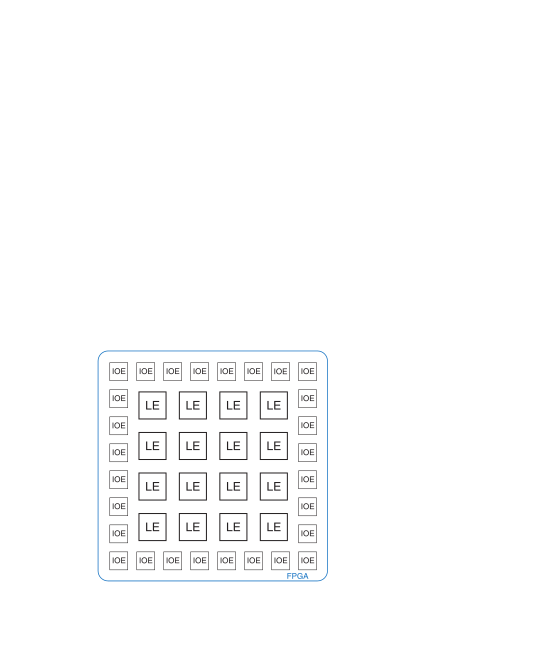
\includegraphics[width=\textwidth]{fpga.pdf}
    \caption{General \acrshort{fpga} layout \cite{harris_digital_2015}}
    \label{fig:fpga}
\end{figure}
%
%
\section{CNN optimizations on FPGA} \label{sec:opti_dataflow}
%
%
The previous section \ref{sec:concept} provides a general layout of what is an \acrshort{fpga} and how does it work. Now, we focus our interest in the design development of a \acrshort{cnn} and what optimizations can be made to perform an efficient inference.

The convolution requires loading weights and pixels into the \acrshort{fpga} and using them to compute the output results. According to \textcite{chen_eyeriss_2017}, the data movement can often be more energy-consuming than actual computation. Smart memory management is then required to implement \acrshort{cnn} on low power device such as \acrshort{fpga}. We discover in this section various techniques for handling the Datapath on the \acrshort{fpga}.
%
\section{Datapath Optimization} \label{sec:dtptopti}
blabla

%
%
\section{Depthwise separable convolution inference on FPGA} \label{sec:inf_fpga}
%
%
\subsection{DSC} \label{subsec:impl_dsc}
%
%
Two studies of the implementation of the \acrshort{dsc} appeared to be relevant: \textcite{bai_cnn_2018, liu_fpga-based_2019}. They present an \acrshort{fpga} accelerator that implements both standard and \acrshort{dsc}. Networks like MobileNetV2 use both convolutions, the first one for keeping as much information as possible, the second one to speed up the inference. 

They both use a commonly used \acrshort{dl} architecture that is called a heterogeneous system: a \acrshort{cpu} which controls the memory accesses and an accelerator that computes the convolution \cite{liu_fpga-based_2019}. The accelerator is designed in such a way that it can perform each layer of the network.

The accelerator in each work has the same structure. The accelerator uses weights, input, and output buffers. To use the same accelerator for both convolutions, they first compute an element-wise multiplication followed by an adder tree. The pattern of additions varies between the studies. 

On one side, \textcite{bai_cnn_2018} divide depthwise and pointwise convolution. As the element-wise multiplication produces a cuboid, we only have to sum either in the spatial or channel axis, either all the cuboid pixels to perform the desired convolution. 

On the other side, \textcite{liu_fpga-based_2019} perform both convolutions using the same adder tree. The dataflow to feed the adder tree depends then on the convolution. However, to use the same structure for both convolutions, it must fill some registers with zero-value (the \acrshort{dsc} has fewer arithmetic operations if we use the same structure we adapt it to the worst case).

To improve the throughput of the network, they use a ping-pong buffer for the weight. Instead of using one buffer that stores the data for convolution, they use two buffers. Alternatively, one fetches weights for the next tile while the other is used for convolution. An illustration is found in Figure \ref{fig:ping_pong_buffer}.
%
\begin{figure}[H]
	\centering
	\includegraphics[width=\linewidth]{pingpong.pdf}
	\caption{Weight buffer in ping-pong structure, from \cite{bai_cnn_2018}}
	\label{fig:ping_pong_buffer}
\end{figure}

Moreover, \textcite{liu_fpga-based_2019} used the roofline model as a method for design space exploration.
%
%
\subsection{Pruning} \label{subsec:impl_prun}
%
%
When implementing a pruned \acrshort{cnn} on an \acrshort{fpga}, we must address the problem of sparsity to keep the parallelism and the performance of the \acrshort{fpga} \cite{zhu_efficient_2020}. As a regular data access pattern is assured by applying a structured pruning scheme, there are some sources of inefficiency that an implementation must handle.

First, the \acrshort{pe}s must avoid performing computation involving 0 weights. \textcite{kang_accelerator-aware_2020} fetches $N_{par}$ data in the channel axis and the $N_{non-zero}$ weights corresponding to the fetched group. A multiplexer is used to choose the pixels associated with non-zero weights. An improvement can be made by avoiding 0 value pixels. \textcite{zhu_efficient_2020} clock gated the computation involving pixels with 0 value to save energy.

Second, to reduce the storage utilization, the zero-weights in a kernel must be discarded. The weights must be encoded in such a way that we keep both values and index of the weights to reduce the overhead of computing the output address.  Usually, kernels are encoded in a format derived from the \acrfull{csr} \cite{mao_exploring_2017}. For example, \cite{zhu_efficient_2020} modified the format to compress further and accelerate the inference.

Finally, the problem of \textbf{load-imbalance} can arise if the number of non-pruned weights is different in each \acrshort{pe} \cite{kim_zena_2018}. Therefore some \acrshort{pe} can finish before another one and it can lead to inefficiency. \textcite{zhu_efficient_2020, kang_accelerator-aware_2020} solved this by setting a uniform number of weights in each kernel or group of fetching weights.


\fbox{\parbox{ \linewidth \fboxrule \fboxsep }{ \textbf{Conclusion about the implementation of \acrshort{cnn} on \acrshort{fpga}}:

\vspace{5mm}
balbla
}}
